\section{Introduction}
\label{sec:intro}

%%需要调研的部分:解答的问题,为什么我们关注多核的scalability问题。随着分布式系统的广泛普及,企业和用户的通用的做法是通过堆积更多的机器来获取更快的处理效率和速度。但是机器堆积的越多,网络带宽,耗电也越来越多,如何充分利用单台机器的多核资源成为很重要的课题。

%一方面,随着多核机器的广泛普及,如何充分利用多核资源成为非常重要的课题,另一方面,现有的很多我们希望充分利用单台机器上的资源,

%目前的现状,需求
As the prevalence of multicore chips, it is foreseeable that tens to hundreds (even thousands) of cores on a single chip will appear in the near future\cite{Borkar2007core}.
However, utilizing multicore sources is still challenging because of the difficulties of parallel programming.
Specifically, traditional parallel programming techniques require the programmer to manually manage synchronization, load balancing and locality, and explicitly understand the detail of underlying hardware, which is error-prone and complicated. %requests the programmer to understand the detail  of underlying hardware.
An alternative approach is dependent on a runtime system for concurrency management. 

%MapReduce以及Phoenix
MapReduce\cite{dean2004mapreduce} is a promising programming model for clusters to perform large scaled datasets processing in a simple and efficient way.
In most cases, programmers only need to implement two functions: 
map function which processes the input data and produce  a series of key-value pairs, and reduce function which is used to aggregate values with the same key.
%Therefore, the programmer dose no need to control synchronization, schedule tasks and fault tolerance manually.
While initially MapReduce is implemented on clusters, Ranger et al. have implemented a MapReduce library for multicore and multiprocess system--Phoenix\cite{ranger2007phoenix}, which demonstrates the feasibility of running MapReduce applications on shared memory multicore machines.
After that, Phoenix is heavily optimized by Yoo et al\cite{yoo2009phoenix2} to obtain better scalability on shared-memory system.
Other libraries such as Metis\cite{mao2010metis} , Tiled-mapreduce\cite{chen2010tiled} and MRPhi\cite{lu2013mrphi} attempt to improve performance of Phoenix from various aspects.


%Other libraries such as Metis\cite{mao2010metis} , Tiled-mapreduce\cite{chen2010tiled} and MRPhi\cite{lu2013mrphi}, also show that MapReduce is a promising programming model for multicore platforms to take full advantage of processing resources.

%The runtime system spawns multiple threads that apply these functions concurrently across the elements of the input dataset. 


%The runtime spawns multiple threads to worker and 
%automatically manages synchronization, load balancing, 
%and locality in order to achieve efficient execution.
%which aggregates values in the key-value pairs according to the key.


\begin{figure}[!h!t]  
	\centering
	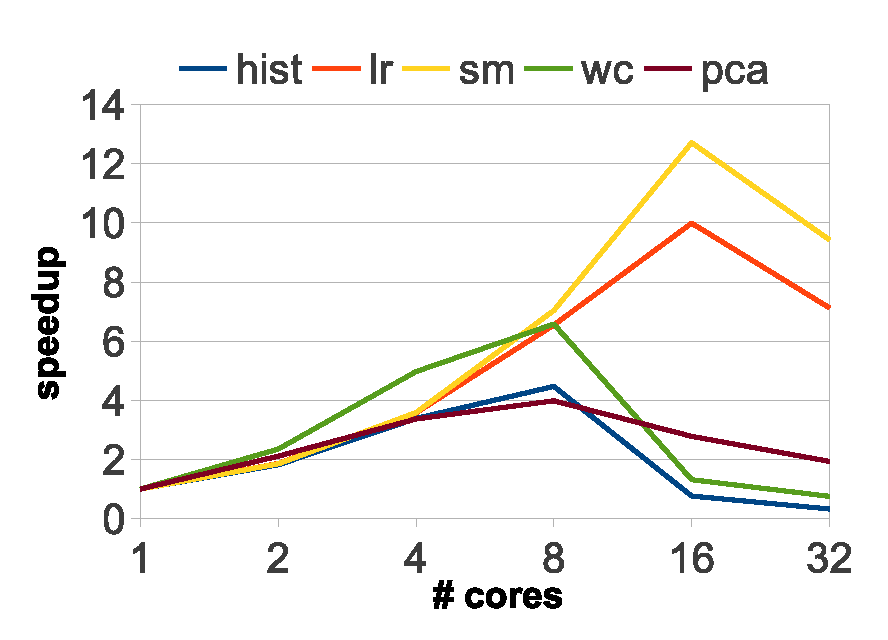
\includegraphics[width=0.45\textwidth]{eps/phoenix_speedup.eps}
	\caption{speedup of Phoenix}
	\label{fig:phoenix:speedup}
\end{figure}

%Due to scale operating systems fo lager-scale, shared-memory systems.
%Phoenix存在的问题
Phoenix exploits shared-memory threads (i.e., Pthread library) to implement parallelism, and the runtime binds each worker to a thread.
Ideally, adding more threads and cores to the system will bring a linear decreasing in execution time.
However, we note that the optimized Phoenix \cite{yoo2009phoenix2} scales worse on a 32-core Intel 4× Xeon E7-4820 system running Ubuntu 12.04 with kernel 3.2.14.
Figure \ref{fig:phoenix:speedup} shows the speedup of the optimized Phoenix runtime.
% which is measured on our 32-core system (the detail of this system will be given in Section \ref{sec:eval}). 
We observe that despite the Phoenix runtime is able to process these applications in parallel, none of them scales well beyond 16 cores and most of them actually degrade when the number of cores exceeds 8.
%While the optimized Phoenix\cite{yoo2009phoenix2} performed well on a 256-thread NUMA system, we find that the runtime significantly underperformed on an 4-chip, 32-cores system running x86 Linux.
%This work focuses on improving Phoenix in the term of scalability and performance from a new perspective.
Since the Phoenix runtime implements multithreading based on shared-memory Pthreads, all threads of the runtime have to share a single address space, which will lead to contention on the single lock \cite{clements2013radixvm}.
As a result, the scalability of applications with Phoenix will be limited. 
%Multithreaded applications on many-core processors can be bottlenecked by contended locks inside the operating system’s virtual memory system.
% where all threads of an application share a single address space, shared address space has a cost, which will limit the scalability of these applications.
 

%However, the benefits of adding more cores will be reduced due to overhead associated with the additional threads----the contention of lock.

%Compared to the cluster version, MapReduce on multicore is able to take ad-
%vantage of fast inter-task communications in shared memory, thus
%avoids the expensive network communications among tasks.
 
%This is the result of the high contention when utilizing threads across multiple chips. We explain these issues in detail in Section 3.
%Hence, with the continuously increasing number of cores, it can easily cause resource pressures on the runtime, operating systems and the CPU caches, which could significantly degrade the performance. 


%Phoenix uses the pthread library to assign tasks among CPU cores and relies on shared memory to handle inter-task communications.

%Phoenix存在的问题,scalability较差的原因
%This work focuses on improving Phoenix in the term of scalability and performance.
%On the one hand, while the original Phoenix performed well on small-scale systems, we found that the runtime significantly underperformed on large-scale systems with multicores.
%Specially, the performance will be better 
%when the number of cores increases from 1 to 4, 
%while the performance will be worse if using more than 4 cores. 
%On the other hand,
%there is a strict barrier between the Map and the
%Reduce phase, which is bad for pipeline and hardware resource utilization.
%To achieve scalable performance while retaining the simplicity of the runtime-based approach, it becomes crucial to address these issues.

%In contrast, Phoenix is a shared-memory version of MapReduce targeted for multi-core and multiprocessor systems.
%Phoenix uses shared-memory threads to implement parallelism.
%Ideally, adding more threads and cores to the runtime would bring about a linear decrease in execution time.
%However, the benefits of adding more cores will be reduced due to overhead associated with the additional threads----the contention of lock.
%Due to parallel programming model is shared-memory multithreading, 
%where all threads of an application share a single address space. 
%A common parallel programming model is shared-memory multithreading, 
%where all threads of an application share a single address space. 
%This shared address space has a cost, which will limit the scalability of these applications. 
%All of these operations are synchronized by a single per-process lock. 




%我们如何解决这个问题
%为了改进Phoenix存在的这些问题,我们提出了一个scalable mapreduce库,它即具有较好的性能,且具有较好的scalability.

%To remedy the above problems, we propose a modified MapReduce architecture in which Map and Reduce phase are pipelined to improve the performance, while preserving the programming interfaces of previous MapReduce frameworks.
To remedy the problems mentioned above, we design a modified MapReduce framework with preserving the programming interfaces of previous MapReduce.
Firstly, we propose a scalable thread libray (\myth).
Then based on \myth, this paper presents a modified MapReduce model for multicore, \myds (Scalable MapReduce), which can efficiently scale on multicore system.

%\myds reserves the similar Phoenix programing interfaces as well.
The main contributions of this paper are concluded as follows:
%Specifically, this paper make the following contributions:
\begin{itemize}
  \item We analyze the important roadblocks that limit scalability of the Phoenix runtime on shared-memory systems. Specifically, we find that the shared address space for multiple threads will be a crucial issue at multicore system.
  
  \item We develop a scalable thread library, \myth, in which threads run in  the separated memory space to avoid the contention on the shared space. Furthermore, \myth provides the \codet{shared-channel} for the threads to communicate with each others. 

  \item Base on \myth, we propose a scalable MapReduce model, \myds.
  And \myds pipelines the Map and Reduce phase by adapting a new producer-consumer model, in which producer does not have to wait when the buffer is full. 

  \item We implement a prototype of \myth and demonstrate the effectiveness of \myds runtime on a 32-cores system. 
%  The optimized runtime exhibits significantly improved scalability over the Phoenix; For 32cores, the new runtime improves speedup up to maximum 5.0x.
\end{itemize}

%介绍文章的组织结构
In order to ground our discussion, we present an overview of MapReduce framework and Phoenix in Section \ref{sec:back}. 
We then develop the design of \myth in Section \ref{sec:design}, focusing on implementing mechanism of extension in \myth. 
%In Section 4 we show how \myth can support
%\myds and illustrate
%the potential benefits of that producer-consumer model for MapReduce framework.
In Section \ref{sec:runtime}, we describe our support for pipelineing map and reduce, and illustrate the potential benefits of the producer-consumer model for MapReduce framework.
We give initial performance results in Section \ref{sec:eval}. 
Related and future work are covered in Sections \ref{sec:rela} and \ref{sec:concl}.

%This paper is organized as follows. In section 2, we review
%the background. Section 3 briefly describes the problems.
%Section 4 presents the experimental setup. Section 5 discusses
%the results in terms of execution time and total power
%consumption. Finally, Section 6 concludes the paper.


%as depicted in
